% This is auto-generated file: do not edit!
% Exported from microMathematics, version 1.19


Данное приложение является мощным
математическим калькулятором,
который основан на работе с
интерактивными документами.
Приложение содержит один рабочий
лист, его можно изменять,
вычислять, сохранять на SD карту,
а также экспортировать в документ
LaTeX или изображение.

Рабочий лист - это полноценный
документ с текстом, формулами и
графиками. Математические объекты
в нём можно редактировать и
вычислять в том виде, как они
выглядят на экране.

Доступны следующие типы объектов:
формула, текстовый результат,
график функции, текстовое поле и
изображение. В данном разделе
даётся краткое описание того, как
работать с этими объектами.

\subsection{Редактирование}

Большинство объектов содержат
поля, которые можно редактировать.
Для редактирования используйте
кнопки на нижней панели
инструментов, с их помощью можно
вводить математические символы в
поля объекта.

Символы с этой панели также можно
ввести и с клавиатуры. Чтобы
узнать символ, соответствующий
кнопке, посмотрите подсказку,
всплывающую при долгом нажатии на
кнопку.

При долгом нажатии на часть
формулы активируется контекстное
меню. В нём выбранную часть можно
удалить, скопировать в буфер
обмена, заменить выражением из
буфера, а также вставить после неё
оператор или функцию, используя
панель инструментов или
клавиатуру.

Для отмены неудачного действия
можно использовать команду
главного меню ''Отменить ввод'':
\begin{center}\begin{tabular}{c} 
\includegraphics[resolution=320]{graphics/how_to_use_fig1.png} \end{tabular}\end{center}

\subsection{Формула}

Формула определяет константу,
интервал, или функцию. Для
добавления формулы используйте
кнопку ''Вставить'' на верхней
панели инструментов
\begin{center}\begin{tabular}{c} 
\includegraphics[resolution=320]{graphics/how_to_use_fig2.png} \end{tabular}\end{center}

или кнопку ''Вставить формулу'' на
нижней панели:
\begin{center}\begin{tabular}{c} 
\includegraphics[resolution=320]{graphics/how_to_use_fig3.png} \end{tabular}\end{center}

После этого появится объект с двумя
пустыми полями, обязательными для
заполнения:
\begin{center}\begin{tabular}{c}
  ${\Box} := {\Box}$
\end{tabular}\end{center}

В левом поле объекта вводится имя
формулы. Имя должно содержать
только буквы или цифры и может
быть использовано далее в других
формулах.

Из верхней панели инструментов
можно вызвать окно ''Свойства
документа'': 
\begin{center}\begin{tabular}{c} 
\includegraphics[resolution=320]{graphics/how_to_use_fig4.png} \end{tabular}\end{center}

В зависимости от параметра
''Разрешить переопределение
формул'', доступного в этом
диалоге, возможны два режима:

а) Если переопределение формул не
разрешено, то имя формулы должно
быть уникальным для всего
документа и эту формулу можно
использовать как до, так и после
её определения.

б) Если переопределение разрешено,
то можно определить несколько
формул с одним и тем же именем, но
при ссылке на неё будет
использован самый последний
вариант, определённый перед
вызывающим объектом.

\subsubsection{Формула - константа}

Если имя формулы не содержит
аргумента в круглых скобках, то
такая формула определяет константу
или интервал. Константа задаёт
какое-либо одно число, которое
определяется правой частью:
\begin{center}\begin{tabular}{ccc}
  $N := 200$ &
  $Sq2 := \sqrt{100} $ &
  $Pi2 := \frac{{\pi}}{2}$ \cr
\end{tabular}\end{center}

Последний пример демонстрирует
использование встроенной константы
пи. Пока доступны следующие
встроенные константы:
\begin{center}\begin{tabular}{ccc}
  ${\pi} = 3.14159$ &
  $pi = 3.14159$ &
  $e = 2.71828$ \cr
\end{tabular}\end{center}

В правой части можно также
использовать любую константу,
определённую ранее:
\begin{center}\begin{tabular}{c}
  $NPi2 := N \cdot Pi2$
\end{tabular}\end{center}

\subsubsection{Формула - интервал}

Формула интервального типа задаёт
переменную, которая изменяется в
заданном интервале с определённым
шагом. Эта переменная служит для
задания аргументов функции при
построении графиков или выводе
таблиц значений.

Для того чтобы задать интервал, в
левом поле введите его имя, а в
пустом правом поле введите символ
'':'' или нажмите на кнопку
''Интервал'' на нижней панели
инструментов:
\begin{center}\begin{tabular}{c} 
\includegraphics[resolution=320]{graphics/how_to_use_fig5.png} \end{tabular}\end{center}

Первый элемент с индексом 0
определяет начальное значение,
второй элемент с индексом 1
определяет следующие значение, а
третий элемент задаёт конечное
значение интервала:
\begin{center}\begin{tabular}{c}
  $x := \left[ 0,\, 0.1 \,..\, 10 \right]$
\end{tabular}\end{center}

Обращаться к элементам интервала
можно следующим образом:
\begin{center}\begin{tabular}{ccc}
  $x \left( 0\right)  = 0.0$ &
  $x \left( 1\right)  = 0.1$ &
  $x \left( 100\right)  = 10.0$ \cr
\end{tabular}\end{center}

Шаг определятся как разница второго
и первого элементов:
\begin{center}\begin{tabular}{c}
  $x \left( 1\right)  - x \left( 0\right)  = 0.1$
\end{tabular}\end{center}

К примеру, задать интервал с
нулевым начальным значением и
содержащий N точек, равномерно
распределённых с шагом ''dy'', можно
таким образом:
\begin{center}\begin{tabular}{cc}
  $dy := 0.05$ &
  $y := \left[ 0,\, dy \,..\, dy \cdot \left( N - 1 \right) \right]$ \cr
\end{tabular}\end{center}

\subsubsection{Формула - функция}

Функция определяет зависимость
между одним аргументом и областью
значений, где каждое значение
аргумента даёт нам только одно
итоговое значение функции.

Имя функции и её аргумент (в
круглых скобках) указываются в
левом поле. Переменную,
обозначающую аргумент, не
обязательно определять ранее -
можно использовать любое
обозначение, содержащее буквы и
цифры:
\begin{center}\begin{tabular}{c}
  $f(t) := sin \left( t\right)  \cdot cos \left( t\right)  / 2$
\end{tabular}\end{center}

Правая часть такого объекта
содержит математическое выражение
для вычисления функции. Если
правая часть не содержит аргумент
из левой части, то такая функция
будет интерпретироваться как
константа.

В правой части можно использовать
другие функции, как встроенные,
так и определённые ранее. Для
этого введите имя функции, затем
символ ''('', а затем её аргумент.
Аргумент также может быть формулой
с любыми операторами и функциями.

\subsection{Текстовый результат}

Этот элемент предназначен для
просмотра результатов вычислений в
текстовом виде: как одно число или
как массив чисел. Для добавления
этого элемента используйте кнопку
''Вставить'' на верхней панели
инструментов или кнопку ''Вставить
текстовый результат'' на нижней
панели:
\begin{center}\begin{tabular}{c} 
\includegraphics[resolution=320]{graphics/how_to_use_fig6.png} \end{tabular}\end{center}

После этого появится объект с двумя
пустыми полями, где левое поле
необходимо заполнить:
\begin{center}\begin{tabular}{c}
  ${\Box} = {\Box}$
\end{tabular}\end{center}

Левое поле может содержать любое
математическое выражение, а в
правом будет показан результат
после нажатия плавающей кнопки
''Вычислить''.

В левом поле можно использовать
любые константы и функции, как
встроенные, как и определённые
ранее:
\begin{center}\begin{tabular}{c}
  ${e}^{{\pi}} \cdot f \left( NPi2\right)  = 2.27286E-14$
\end{tabular}\end{center}

Если левая часть не содержит
переменных интервального типа, то
результатом вычислений будет одно
число:
\begin{center}\begin{tabular}{c}
  $y \left( N - 1\right)  - y \left( 0\right)  = 9.95$
\end{tabular}\end{center}

Если же слева используется
интервал, то результат будет
массивом чисел, соответствующих
интервалу. Ввиду ограниченности
дисплея, будут показаны только
шесть первых и последнее число из
этого массива:
\begin{center}\begin{tabular}{c}
  $x = [0.0, 0.1, 0.2, 0.3, 0.4, 0.5, ..., 10.0]$
\end{tabular}\end{center}
\begin{center}\begin{tabular}{c}
  $2 \cdot y = [0.0, 0.1, 0.2, 0.3, 0.4, 0.5, ..., 19.9]$
\end{tabular}\end{center}

Количество показанных элементов, а
также режим вычисления и показа
поля результата можно изменить в
настройках формулы. Для вызова
окна настроек необходимо выделить
всю формулу целиком, после чего
появится плавающая кнопка
''Настройки объекта'', по нажатии на
которую и откроется окно настроек:
\begin{center}\begin{tabular}{c} 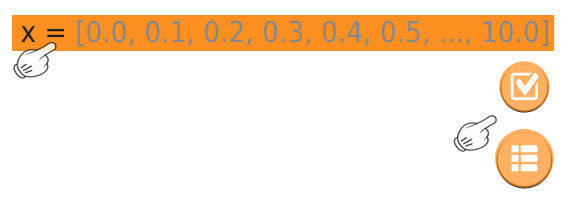
\includegraphics[resolution=320]{graphics/how_to_use_fig7.png} \end{tabular}\end{center}

Также появится вторая плавающая
кнопка - ''Подробности''. При
нажатии на неё откроется окно, где
будут показаны все элементы
массива.

Обратите внимание, что данная
версия программы не поддерживает
использование двух и более
переменных интервального типа в
объекте текстового результата.

\subsection{График функции}

Данный элемент предназначен для
отображения графика функции одной
переменной. Для добавления
используйте кнопку ''Вставить'' на
верхней панели инструментов или
кнопку ''Вставить график функции''
на нижней панели:
\begin{center}\begin{tabular}{c} 
\includegraphics[resolution=320]{graphics/how_to_use_fig8.png} \end{tabular}\end{center}

Появится поле графика с шестью
пустыми полями. Функция, для
которой строится график, задаётся
в левом среднем поле, а аргумент
функции указывается в нижнем
среднем поле:
\begin{center}\begin{tabular}{c} 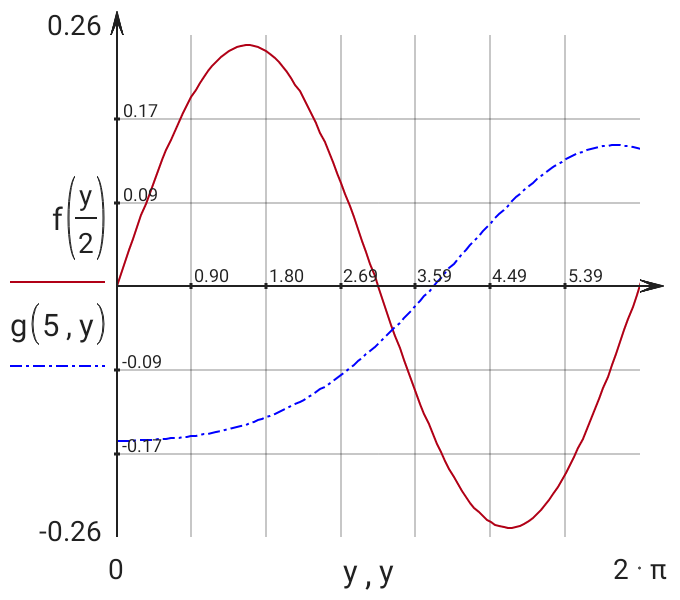
\includegraphics[resolution=320]{graphics/how_to_use_fig9.png} \end{tabular}\end{center}

Для более подробного ознакомления с
графиком функции см. примеры
''График функции'' и ''Полярный
график'' из навигатора приложения.

\subsection{Текстовое поле}

Этот элемент служит для ввода
простого текста. Добавить
текстовое поле также можно по
команде главного меню ''Вставить''
или кнопкой ''Вставить текстовое
поле'' на нижней панели
инструментов:
\begin{center}\begin{tabular}{c} 
\includegraphics[resolution=320]{graphics/how_to_use_fig10.png} \end{tabular}\end{center}

Если при помощи контекстного меню
''Выбрать всё'' выделить весь текст
фрагмента, то  появится плавающая
кнопка ''Настройки объекта''. 

При нажатии на эту кнопку
откроется окно настроек текста,
где можно изменить его стиль и
нумерацию. Например, заголовки
глав в данном документе  имеют тип
''Глава'' со включенной
автоматической нумерацией.

\subsection{Изображение}

Если есть файл с изображением,
которое хотелось бы внедрить в
документ в виде иллюстрации, то
это также можно сделать. Для этого
нужно выбрать кнопку ''Вставить'' на
верхней панели инструментов или
кнопку ''Вставить изображение из
файла'' на нижней панели:
\begin{center}\begin{tabular}{c} 
\includegraphics[resolution=320]{graphics/how_to_use_fig11.png} \end{tabular}\end{center}

После этого откроется окно
настройки изображения, где можно
выбрать нужный файл и задать
желаемые размеры.

Программа поддерживает файлы
следующих форматов: png, bmp, gif,
jpeg, svg.

Если в окне настроек установить
флаг ''Внедрить в документ'', то
изображение будет сохранено внутри
документа. Это увеличивает размер
файла документа, но позволяет его
использовать в дальнейшем, даже
если файл с изображением будет
удалён.

Если же флаг ''Внедрить в документ''
не установлен, то внутри документа
будет сохранён только путь к
файлу. В этом случае, файл с
изображением нужно всегда
копировать вместе с документом.

Свойства внедрённого изображения
можно изменить. Для этого долгим
нажатием на картинке дождитесь
появления плавающей кнопки
''Настройки объекта'', при нажатии
на которую появится окно со
свойствами этой картинки.